%DESIGN OVERVIEW
\subsection{Steganography and WebStegFS}
% Figure 1: Original
% Figure 2: lsbsteg encoded image
% Figure 3: other encoded image
% Figure 4: detection % chart
% Figure 5: visual encoding evidence


The primary purpose in a web based covert file system is confidentiality and plausible deniability. Using steganography can provide both confidentiality for users as well as plausible deniability. However, steganography also has risks that make it vulnerable to both. Steganalysis and visible alterations\cite{PierreRicher2003} can make steganography detectable, thus removing the aspect of both confidentiality and plausible deniability. However, there are ways to reduce the risks of using steganography. 

\subsubsection{Risks Using Steganography}
%Not enough data

The greatest risk to using steganography, particularly our steganography module, is that an embedded message can be discovered using statistical analysis. Since the original images exist on Tumblr and can be retrieved using the Cat API, our images that get uploaded to Sendspace can be compared to the originals. Statistical analysis between the original and the modified images will indicate that a message has been embeded. There are alternative steganograhpy techniques available, but there is still several steganalysis tools available for detection of these various steganography techinques~\cite{Laden}. For example, Virtual Steganography Laboratory (VSL) is a tool developed by Michal Wegrzyn and Pawel Forczmanski, of West Pomeranian University of Technology. VSL has a simple GUI that allows users to select an image and run certain steganalysis modules on that image. The results of the analysis is outputted to an easy-to-read csv file. Figure 1 is the original image used. Figure 2 is a modified image with 2.75 KB of data encoded into it using our custom steganography module. Figure 3 is a modifed image with the same 2.75 KB of data encoded into it using VSL's least significant bit steganography module.
\begin{figure}[h]
	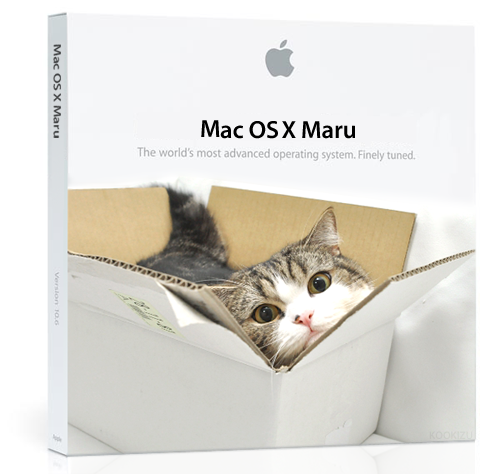
\includegraphics[width=2.5in]{smalloriginal}
	\caption{Original image}
\end{figure}
\begin{figure}[h]
	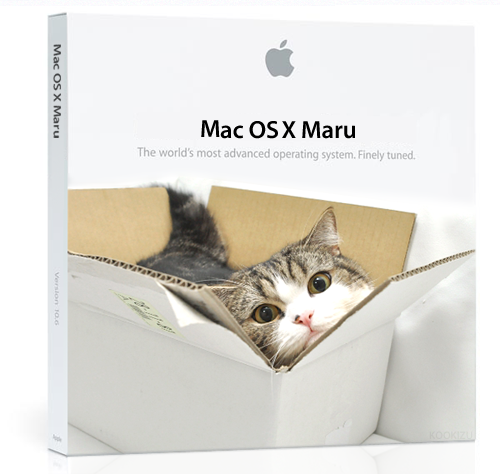
\includegraphics[width=2.5in]{smallmodifiedOURS}
	\caption{Image encoded with a 2.75 KB message using our steg module}
\end{figure}
\begin{figure}[h]
	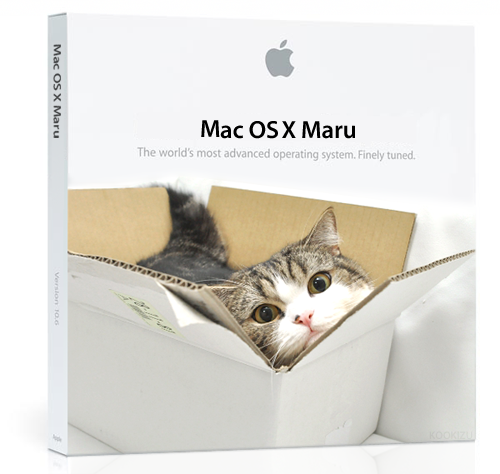
\includegraphics[width=2.5in]{smallmodifiedTHEIRS}
	\caption{Image encoded with a 2.75 KB message using VSL's steg module}
\end{figure}
The steganaylsis tools, provided by VSL, determines that the there is a 1.34 KB message encoded into the original image. In reality there is no message encoded into the original, but this value offers a baseline of comparison with images that are modified. VSL determines that the image modified using our steganography module has a 1.75 KB message encoded into it. VSL also determines that the image modified using the VSL steganography module has a 3.60 KB message. Figure 4 summarizes these results.
\begin{figure}[h]
	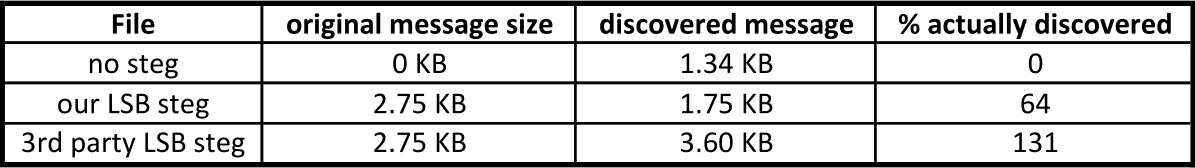
\includegraphics[width=3in]{steganalysis}
	\caption{Table summarizing results of steganalysis}
\end{figure}
These results are significant because VSL is able to detect substantial changes in the images that are modified. The steganalysis shows that there is likely a message inside both modified images when the images are compared against the original image. Not only can steganalysis detect changes caused by multiple implementations of least significant bit steganography, but the changes can be visually apparent as well. Figure 5 shows both an encoded image and its original.
\begin{figure}[h]
	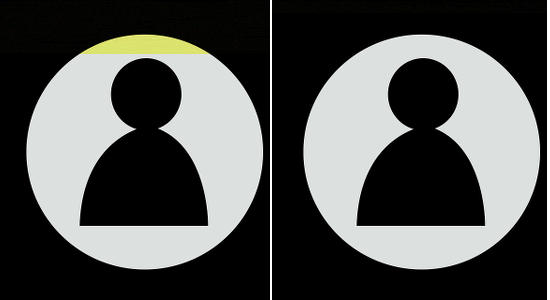
\includegraphics[width=2.5in]{comparison}
	\caption{Left: encoded, Right: original}
\end{figure}
In some cases, our implementation of least significant bit steganography can cause a significant amount of discoloration in images. The white portions in figure 5 turn yellow when data is encoded into those pixels. 

\subsubsection{Mitigating Risks of Steganography}
%Not enough data
These risks are mitigated by the fact that there is no universal standard for steganography methods. A user can easily replace the steganography module that we offer with a module of their own. That way, even if someone knows an image is not the original, that person will still not know who encoded it, or what kind of module was using for the encoding. Also, an encryption module can easily be added to our application and used to encrypt messages before they are encoded into an image. So even if someone knows what kind of steganography module is being used to encode messages into images, that person will also have the added challenge of decrypting the information. There is no research to indicate that encryption helps in fooling steganalysis tools, and it most likely would indicate stronger evidence of steganography. Finally, since the original images exist on the internet, it will limit the plausible deniability of the user. It can be called into question as to why a certain user is uploading images that do not belong to that user to an online image database. 

%IMPLEMENTATION SECTION
\subsection{Encoding a File System}

The covert file system uses a drop in steganography module that takes in a bytearray object and returns a URL to an image. We used "least significant bit" steganography for this application because of its simplicity and reliability.

\subsubsection{Steganography Implementation}

Least significant bit (LSB) steganography is a Substitution type of steganography~\cite{Nosrati2011} that replaces the least significant bits in the image's pixels. Our steganography module is not true LSB steganography because we replace multiple bits in each pixel allowing us to encode one byte of data into every pixel. We designed our steganography technique this way to decrease the amount of images required to encode large file systems at the cost of only minimal discoloring. 

First, we break every byte of the message into three segments. Two segments of the byte will contain three bits, and the last segment will contain two bits. Next, we replace the three least significant bits of the red component with the first three bit segment. The green component follows, with the replacement of its least significant bits with the second three bit segment. Lastly, we replace the two least significant bits of the blue component with the remaining two bit segment of data. 

There are obvious drawbacks to our implementation of LSB steganography, primarily that the image may appear distorted as seen in Figure 5 and CovertFS images are X percent easier to detect using standard statistical analysis techniques compared to true LSB steganography as seen in figure 4. However, this implementation enables us to store more bytes than other implementations of LSB steganography which decreases the latency in uploading and downloading images in large file systems [? Need evidence].
 
\subsubsection{File System to Images}

%David, I will need you to describe how the FUSE file system is prepared for encoding. Additionally, I will need information on how the files are uploaded as they are added to the file system (and future parallel upload/download). 
In order to encode a message (either the contents of a file, or the string that represents the entire file system), we must start with an image. We use "The Cat API" which retrieves a random cat picture from the web~\cite{CatAPIDoc}. Once we retrieve the image, we determine the number of bytes we can encode in the image by finding the area of the image in pixels. Since we encode one byte per pixel, the total number of bytes we can encode is height \textit{x} width, \textit{n} bytes. For example, a 640x480 pixel image can hold 307,200 bytes of data. Appending a special end of file byte encoding allows us to read the pixels only until the end of the file. After appending the EOF, we break the data into two sets, one set containing the last \textit{n+1} bytes and the other set, the remaining bytes. This allows us to encode the final bytes of data in the first image, the next to final bytes in the second, and so on, so that the final image we encode has a pointer to the next. We are creating a linked list of images as we go.

Encoding a file into an image is simple-- we take the data of the image, which is already stored as a byte string, and send it to the encoder. The file system is handled differently. When encoding the file system, we first create a string-- it is similar to a comma-separated value file, but it uses commas, spaces, and newline characters to delineate between a single file's name and info, different files, and different directories. By using the same standard for encoding and decoding this string, we are able to recreate the same file system in a different place, after saving to a string. Once the file system is saved to a string, it is converted to a byte string and sent to the steganography class for encoding and upload.